\documentclass[12pt]{article}
\usepackage[english]{babel}
\usepackage[a4paper]{geometry}
\usepackage{graphicx}
\usepackage{amsfonts}
\usepackage{amsmath}
\usepackage{amssymb}
\usepackage{breqn}
\usepackage[]{fancyhdr}
\usepackage{tikz}
\usepackage{subcaption}
\usepackage{xcolor}
\usepackage{hyperref}
%\usepackage{times}
%\usepackage{merriweather}
%\usepackage{draftwatermark}
\usepackage[backend=bibtex, style=ieee]{biblatex}

\addbibresource{draft.bib}

\usetikzlibrary{decorations}
\usetikzlibrary{snakes}

%\newcommand{\comment}[1]{{\color{red}[\textbf{comment:} #1 ]}}


\pagenumbering{arabic}
\numberwithin{equation}{section}
\numberwithin{table}{section}
\numberwithin{figure}{section}


\newcommand{\fww}[0]{\mathcal{F}^{\mathrm{WW}}}
\newcommand{\fdp}[0]{\mathcal{F}^{\mathrm{dipole}}}
\newcommand{\sdp}[0]{\sigma_{\mathrm{dipole}}}
\newcommand{\sdpa}[0]{\sigma_{\mathrm{dipole\,Adj.}}}
\newcommand{\GeV}[0]{\mathrm{GeV}}
\newcommand{\comment}[1]{\texttt{\color{red}#1}}
\newcommand{\pairdot}[2]{ \mathbf{#1}\cdot\mathbf{#2}  }
\author{
T.~Goda,$^1$, K.~Kutak$^{1}$ and S.~Sapeta$^1$\\\,\\
$^1$ 
{\small\it The H.\ Niewodnicza\'nski Institute of Nuclear Physics PAN,}\\ 
{\small\it Radzikowskiego 152, 31-342 Krak\'ow, Poland}\\%\,\\
%$^2$ 
%{\small\it Physics Department, Brookhaven National Laboratory,}\\
%{\small\it Upton, NY 11973, USA}\\
}	 
%\title{ New parameters for the Golec-Beiernat--W\"usthoff and Bartels--Golec-Biernat--Kowlski saturation models in the $k_t$-facorization formula of $F_2$}
\title{Effects of gluon kinematics and the Sudakov form factor on the GBW and BGK saturation models}
\date{\today}

\begin{document}

\maketitle

%--------------- preprint numbers ---------------------
\vspace{-25em}
\begin{flushright}
%  IFJPAN-IV-2022-16\\
\end{flushright}
\vspace{20em}
%-----------------------------------------------------------------

\begin{abstract}
  
\end{abstract}
%%%%%%%%%%%%%%%%%%%%%%%%%%%%%%%%%%%%%%%%%%%
%
%\section{Introduction}
%
%%%%%%%%%%%%%%%%%%%%%%%%%%%%%%%%%%%%%%%%%%%
\comment{Bibliography will be properly made once the draft is complete. For only now I use biblatex.}
%%%%%%%%%%%%%%%%%%%%%%%%%%%%%%%%%%%%%%%%%%

\section{Introduction}
%
%%%%%%%%%%%%%%%%%%%%%%%%%%%%%%%%%%%%%%%%%%
\begin{figure}[t]
\centering
\resizebox{0.75\textwidth}{0.25\textwidth}{
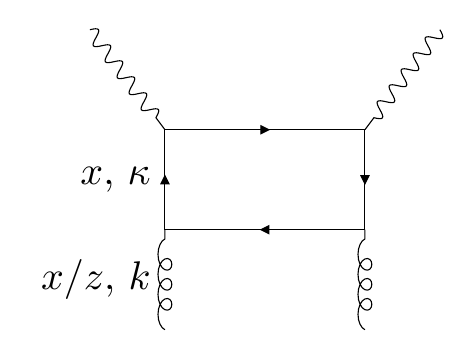
\begin{tikzpicture}
\draw[snake=coil,segment aspect=0,segment length=0.1in](-0.875in , 0.5in)--(-0.5in,0.in);
\draw[snake=coil,segment aspect=0,segment length=0.1in](0.875in ,0.5in)--(0.5in,0.in);
\draw(-0.5in , 0in)--(0.5in,0in)--(0.5in , -0.5in)--(-0.5in,-0.5in)--cycle ;

\filldraw(0.02in,0)--(-0.02in,-0.02in)--(-0.02in,0.02in)--cycle;
\filldraw(-0.02in,-0.5in)--(0.02in,-0.52in)--(0.02in, -0.48in)--cycle;

\filldraw(-0.5in,-0.23in)--(-0.52in,-0.27in)--(-0.48in,-0.27in)--cycle;
\filldraw(0.5in,-0.27in)--(0.52in,-0.23in)--(0.48in,-0.23in)--cycle;

\draw(-0.5in , -0.25in)node[left,scale=0.02in]{$x$, $\kappa$};
\draw(-0.5in , -0.75in)node[left,scale=0.02in]{$x/z$, $k$};
\draw[ snake=coil,segment aspect=1.5,segment length=0.1in](0.5in , -1in)--(0.5in,-0.5in);
\draw[snake=coil,segment aspect=1.5,segment length=0.1in](-0.5in , -1in)--(-0.5in,-0.5in);
\end{tikzpicture}
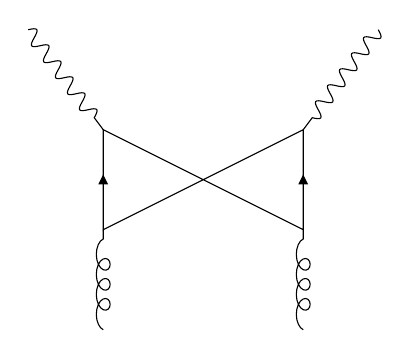
\begin{tikzpicture}
\draw[snake=coil,segment aspect=0,segment length=0.1in](-0.875in , 0.5in)--(-0.5in,0.in);
\draw[snake=coil,segment aspect=0,segment length=0.1in](0.875in ,0.5in)--(0.5in,0.in);
\draw(-0.5in , 0in)--(0.5in,-0.5in)--(0.5in ,0in)--(-0.5in,-0.5in)--cycle ;

\filldraw(-0.5in,-0.23in)--(-0.52in,-0.27in)--(-0.48in,-0.27in)--cycle;
\filldraw(0.5in,-0.23in)--(0.52in,-0.27in)--(0.48in,-0.27in)--cycle;

\draw[ snake=coil,segment aspect=1.5,segment length=0.1in](0.5in , -1in)--(0.5in,-0.5in);
\draw[snake=coil,segment aspect=1.5,segment length=0.1in](-0.5in , -1in)--(-0.5in,-0.5in);
\end{tikzpicture}
}
\caption{Kinematic variables of the gluon contribution to $F_2$. The momentum fraction of gluon is $x/z$ as it has to contribute via the quark box.
}
\label{fig:gluon-kinem}
\end{figure}
%Factorization has played central role in QCD, where one expresses a cross section in terms of factors, each depends on a different scale. Parton Distribution Functions (PDF) are examples of such objects which appear in factorization. The PDFs describe the structure of hadrons, and they are process independent. As PDFs are not perturbatively calculable objects, they have to be obtained from experiments. 
%Deeply Inelastic Scattering (DIS) is one of such experiments which can probe the structure of proton. Process independence means that the PDFs obtained in DIS can be used in other experiments such as proton-proton collision.

In the small-$x$ region of DIS, interactions are dominated by gluons\cite{Kovchegov:2012mbw}. As a photon does not interact directly with a gluon, it interact through a box of quarks as depicted in Fig.~\ref{fig:gluon-kinem}. 
An object, which is central to the description of this process is called dipole gluon density, $\mathcal{F}(x,k_t^2)$, which is a type of transverse momentum dependent PDFs (TMD PDF). This appears in the $k_t$-factorization formula, which we will discuss later, and plays role similar to that of collinear parton distribution function in the collinear factorization.
The dipole gluon density is also called unintegrated gluon density~(UGD) since it is related to the collinear (integrated) gluon density by
\begin{equation}
xg(x,Q^2)=\int^{Q^2}_0 dk_t^2 \mathcal{F}(x,k^2_t).
\end{equation}
Much effort has been made to study this object, notably the work of Balistky, Fadin, Kuraev and Lipatov (BFKL)~\cite{Balitsky:1978ic, Kuraev:1977fs} has predicted sharp rise of cross sections with $1/x$.  However, such rise violates the Froissart bound~\cite{Kovchegov:2012mbw}. The work of Balitsky and Kovchegov (BK)~\cite{Balitsky:1995ub,Kovchegov:1999yj} incorporated the gluon recombination, by including nonlinear term in the evolution, thus taming the growth. The phenomenon described by this nonlinear term is called saturation.
Despite the success of such evolution equations, there are several popular phenomenological models owing to their simplicity. A notable example is the Golec-Biernat--W\"sthoff saturation model~\cite{Golec-Biernat:1998zce}. The model was originally proposed in the position space version of the $k_t$-factorization formula, and the object which corresponds to the gluon density of the $k_t$-factorization is called dipole cross section.
In the GBW model, the dipole cross section has the form~\cite{Golec-Biernat:1998zce}
\begin{align}
\sigma_{\mathrm{dipole}}(x,r)&=\sigma_0\left(1-e^{-r^2/R^2_0}\right)&\mathrm{where}&
&R^{-2}_0&=\frac{Q_0^{2}}{4}\left(\frac{x_0}{x}\right)^\lambda.
\end{align}
%\comment{here I use $R_0$ instead of $Q_s$ since for BGK below, $Q_s\neq 1/R_0$. }
The dipole cross section is related to the gluon density by the Fourier transform: 
\begin{equation}
\alpha_s\mathcal{F}(x,k_t^2)=\frac{N_c}{4\pi}\int\frac{d^2\mathbf{r}}{(2\pi)^2}e^{i\mathbf{k}_t\cdot \mathbf{r} }\nabla_{\mathbf{r}}^2\sigma_{\mathrm{dipole}}(x,r).
\label{eq:dipole-gluon}
\end{equation}
%An important feature of the GBW model is that it describes the phenomenon of saturation in a simple form. 
The essence of GBW model is encoded in the $x$-dependent saturation scale $Q_s^2(x)=Q^2_0(x_0/x)^{-\lambda}$, which separates the saturation region and the scaling region.
A further development was made by Bartels, Golec-Biernat and Kowalski~(BGK)~\cite{Bartels:2002cj} which incorporates the DGLAP evolution by modifying the exponent to 
\begin{equation}
R_0^{-2}=\frac{\pi^2\alpha(\mu^2)xg(x,\mu^2)}{3\sigma_0},
\end{equation}
where
\begin{align}
\mu^2&=\frac{C}{r^2}+\mu_0^2 & &\mathrm{and} & xg(x,Q^2_0)&=A_g x^{-\lambda_g}(1-x)^{5.6},
\end{align}
thus improving the description of data at higher $Q^2$.\\
While these models enjoyed much success in phenomenology of DIS, including the diffractive and photo-production processes~\cite{Golec-Biernat:1998zce,Golec-Biernat:1999qor}, as later discussed in detail, the derivation of the dipole-factorization formula from the $k_t$-factorization involves with certain simplification and introduction of massive light quarks. 
In the rest of this section, differences of the $k_t$-factorization and the dipole-factorization are outlined.  In Sec.~\ref{Results}, results of the new fit to HERA data are presented and discussed. In Sec.~\ref{Dijet process at EIC}, we apply the results to compute corss section for dijet processes in DIS at Electron-Ion Collider (EIC) and make comparisons with Ref.~\cite{vanHameren:2021sqc}.\\

Let us consider the inclusive DIS process $e p\rightarrow \gamma^* (q) p(p)\rightarrow X$. %where a proton and a photon interact, and their momenta are $p$ and $q$ respectively.
Additionally, let us introduce $q'\equiv q+x p$. 
Then one  decomposes $k$ and $\kappa$ (Fig.~\ref{fig:gluon-kinem}) as
\begin{align}
    \kappa&=\alpha p-\beta q'+\kappa_t&&\mathrm{and}& k&=a p- bq'+k_t.
\end{align}
For the contribution depicted in Fig.~\ref{fig:gluon-kinem}, the structure function, $F_2$ for transversely and longitudinally polarized photons, factorize, with a change of variable  ${\boldsymbol{\kappa}'}_t\equiv{\boldsymbol{\kappa}_t}-(1-\beta)\mathbf{k}_t$, in the form~\cite{ Kimber:2001uaa,Kwiecinski:1997ee}
\begin{multline}
	F_2(x,Q^2)=\sum_f e_f^2 \frac{Q^2}{2\pi}\int\frac{dk^2_t}{k_t^2}\int^1_0d\beta\int d{\kappa'}_t\alpha_s(\mu^2) \mathcal{F}(x/z,k_t^2)\Theta(1-x/z)\\
	\left[\left(\beta^2+(1-\beta)^2\right)\left(\frac{I_1}{2\pi}-\frac{I_2}{2\pi}\right)
	+\left(m_f^2+4Q^2\beta^2(1-\beta)^2\right)\left(\frac{I_3}{2\pi}-\frac{I_4}{2\pi}\right)\right],
	\label{eq:angle-integrated}
\end{multline}
where
\begin{equation}
	\frac{1}{z}=1+\frac{{\kappa'}^2_t+m_f^2}{\beta(1-\beta)Q^2}+\frac{k^2_t}{Q^2}.
	\label{eq:z}
\end{equation}
(see Ref.~\cite{ Kimber:2001uaa,Kwiecinski:1997ee} for detail.)
%and
%\begin{equation}
%	\begin{split}
%		\frac{I_1}{2\pi}=\frac{N_1N_2+N_3^2}{\left( N^2_1+2N_1N_2+N_3^2\right)^{3/2}}, &\hspace{1cm}
%		\frac{I_2}{2\pi}=\frac{N_3-(1-2\beta)N_1}{(N_1+N_4)\sqrt{ N^2_1+2N_1N_2+N_3^2}},\\
%		\frac{I_3}{2\pi}=\frac{N_1+N_2}{\left( N^2_1+2N_1N_2+N_3^2\right)^{3/2}},&\hspace{1cm}
%		\frac{I_2}{2\pi}=\frac{(1-\beta)}{(N_1+N_4)\sqrt{ N^2_1+2N_1N_2+N_3^2}},
%	\end{split}
%\end{equation}
%for
%\begin{equation}
%	\begin{split}
%		N_1\equiv\beta(1-\beta)Q^2+m_f^2, &\hspace{2cm}
%		N_2\equiv{\kappa'}_t^2+(1-\beta)^2k_t^2,\\
%		N_3\equiv{\kappa'}_t^2-(1-\beta)^2k_t^2, &\hspace{2cm}
%		N_4\equiv{\kappa'}_t^2+\beta(1-\beta)k_t^2.
%	\end{split}
%\end{equation}
Hereafter, we will call Eq.~(\ref{eq:angle-integrated}) $k_t$-factorizaton formula.

If one, instead, uses $ 1/z=\left(1+4 m_f^2/Q^2\right)$ and assumes that $\mu$ is independent of $\kappa'$ and $k_t$, 
the above formula can be written in the impact parameter space~\cite{Golec-Biernat:1998zce} (i.e. dipole-factorizaton formula)
\begin{equation}
F_2\left(x,Q^2\right)\sim\int^1_0d\beta \int d^2\mathbf{r}\left|\Psi\left(x,\beta,Q^2\right)\right|^2\sigma_{\mathrm{dipole}}\left(x,r\right),
\label{eq:dipole-factorization}
\end{equation}
where the photon wave function, $\left|\Psi\left(x,\beta,Q^2\right)\right|^2$, describes a splitting of the incoming photon into a $q\overline{q}$ pair with light-cone momenta fractions $\beta$ and $1-\beta$ respectively, and the dipole cross section, $\sigma_{\mathrm{dipole}}\left(x,r\right)$, describes the interaction of the colour dipole with the proton.\\

The original GBW and BGK models were fitted in the dipole factorization, Eq.~(\ref{eq:dipole-factorization}). In this study, we use Eq.~(\ref{eq:angle-integrated}), where the gluon density is obtained by evaluating Eq.~(\ref{eq:dipole-gluon}) numerically.
In order to account for the running coupling, we assume that $\alpha_s$ in Eq.~(\ref{eq:dipole-gluon}) is constant for the GBW model, and thus explicitly multiply by running coupling;
\begin{equation}
\alpha_s(\mu^2)\mathcal{F}(x,k_t^2)\rightarrow \alpha_s(\mu)\frac{\alpha_s\mathcal{F}(x,k_t^2)}{0.2},
\end{equation}
where %0.2 is an arbitrary normalization, and 
\begin{equation}
\alpha_s(\mu^2)=\frac{1}{\frac{11 C_A-2n_f}{12\pi}\log\left(\frac{\mu^2}{\Lambda_{\mathrm{QCD}}^2 }\right)},
\end{equation}
and  $\Lambda_{\mathrm{QCD}}^2=0.09\;\GeV^2$.
The factor 0.2 is an arbitrary normalization and the effect is absorbed by $\sigma_0$ and hence, bears no importance.
While there is some ambiguity on what the argument of $\alpha_s(\mu^2)$ should be, we follow Ref.~\cite{Kwiecinski:1997ee} and use
\begin{equation}
	\mu^2=k_t^2+{\kappa'}_t^2+m_f^2+\mu^2_0,
\end{equation}
where we add $\mu^2_0=4\;\GeV^2$ in order to freeze the coupling at low scales.

The GBW and BGK models were fitted to the $F_2$ data from HERA~\cite{Abt:2017nkc}. A numerical program was written with help of CERNLIB~\cite{Kolbig:1972zz}, GSL~\cite{GSL}, CUBA~\cite{Hahn:2004fe} and ROOT~\cite{Brun:1997pa} libraries to evaluate $F_2$. The data were selected to be in the range $0.045\leq Q^2\leq 650\;\mathrm{GeV^2}$, $x<0.01$.
As with the previous fit~\cite{Goda:2022wsc}, the $c$ and $b$ flavours were taken into account with the mass $1.3$ and $4.6\;\mathrm{GeV}$, respectively. As discussed earlier, we take the light quarks to be massless.
The fitting was performed using MnMigrad and MnSimplex of ROOT::Minuit2~\cite{James:2004xla}.

%%%%%%%%%%%%%%%%%%%%%%%%%%%%%%%%%%%%%%%%%%%%%%%
%
\section{Results}
\label{Results}
%
%%%%%%%%%%%%%%%%%%%%%%%%%%%%%%%%%%%%%%%%%%%%%%%
The fit was performed for the following cases
\begin{itemize}
\item GBW model with the fixed coupling in $k_t$-factorization  ($k_t$-GBW),
\item GBW model with the running coupling in $k_t$-factorization (rc-$k_t$-GBW),
\item BGK model in $k_t$-factorization ($k_t$-BGK),
\end{itemize} 
and, as a reference, we provide the following results from Ref.~\cite{Goda:2022wsc};
\begin{itemize}
\item GBW model with massless light quarks in the dipole-factorization ($r$-GBW),
\item GBW model with massive light quarks in the dipole-factorizations ($r$-GBW-massive),
\item  BGK model in  the dipole-factorization ($r$-BGK).
\end{itemize} 

The results of fits are summarized in Tab.~\ref{tab:table}. 
The fit quality of $k_t$-GBW is almost unchanged from $r$-GBW, while rc-$k_t$-GBW shows remarkable improvement, almost halving the $\chi^2$ value.
It was pointed out in Ref.~\cite{Albacete:2004gw,Albacete:2007yr,Albacete:2010sy} that in the BK evolution, the running coupling correction have considerable effects. \comment{What is the connection? Their result regarding the 1/x grad of $Q_s$ becoming smaller is clearly not present in our case. If we consider $\mathcal{F}$ with running coupling, it will be a bit bent in very small-x. besides, the analysis of \cite{Albacete:2004gw} extends to around $Y=\ln(x_0/x)\sim35$. for our case it may be just not low enough. (though around $Y=10$, $\alpha_0=0.2$ and running have sizable difference. ) }
Another notable point is that, except for the normalization $\sigma_0$, the parameters are very similar, particularly those of rc-$k_t$-GBW are almost identical to those of $r$-GBW. This can be seen also in Fig.~\ref{fig:GBW}. \\
Let us analyze the difference in $\sigma_0$. 
Recalling that the difference between the $k_t$-factorization formula and the dipole-factorization formula is in $x/z$, where this enters in the GBW formalism as modified $x$. It is easy to see that, as $x$ grows, the dipole cross section gets suppressed (Keeping in mind the suppression by the photon wave function in the large-$r$ region.). Such effect was discussed previously in Ref.~\cite{Kutak:2004ym} in the context of the BK equation. In fact, this suppression is the motivation given in Ref.~\cite{Golec-Biernat:1998zce} for such modification of $x$, so that in the small-$Q^2$ limit, the total cross section remains finite.    
Since 
\begin{equation}
\left(1+\frac{4 m_f^2}{Q^2}\right)\leq\left(1+\frac{k_t^2}{Q^2}+\frac{{\kappa'}_t^2+m_f^2}{\beta(1-\beta)Q^2}\right),
\end{equation}
the $k_t$-factorization case receives more suppression. Consequently, the normalization factor $\sigma_0$ rises to compensate the suppression. Thus, one would expect that the massive light quarks partially simulate the effect of $x/z$.
It is therefore, interesting to see that the parameters of $k_t$-GBW, are closer to those of $r$-GBW-massive than to the parameters of $r$-GBW.    
However, it seems that there is a compensating factor in rc-$k_t$-GBW. 
The compensating effect can be understood as follows. As it is visible in  Fig.~\ref{fig:GBW}, larger $x_0$ enhances the small-$r$ region which corresponds roughly to the large-$k_t$ of the dipole gluon density which also is visible. 
As the running coupling depends on $k_t^2$,  one can expect that the large-$k_t$ region gets suppressed.  Therefore, one can conclude that the change in $x_0$ is a direct consequence of the running coupling.\\
While the GBW model remains almost unaffected, the BGK model seems to show slightly more change. The difference is more prominent in the small-$x$ region (Fig.~\ref{fig:BGK}), particularly noticeable in the second peak of the gluon density.
The change is cleanly visible in the saturation scale of Fig.~\ref{fig:BGK}. \comment{Is there anything more to be said?}
The resulting $F_2$ of respective models are shown in Figs.~\ref{fig:GBW-Grid}~and~\ref{fig:BGK-Grid}.
While the $r$-GBW and $k_t$-GBW show little difference, rc-$k_t$-GBW clearly shows better fit quality in the high-$Q^2$ region. This is clearly shown in the histogram at the bottom. 
As for the BGK model, the difference is too small to be seen in the top plots. However the bottom histogram shows some differences. While the small-$Q^2$ region is somewhat improved, as a whole, the changes cancel out. 

\comment{notice the $x$-slope of $F_2$ in small-$Q^2$ is affected. Recalling that in $r$-formula that region was controlled by the mass of light-quarks. }
\comment{Also, running GBW is showing somewhat similar pattern with the Sudakov improvement.}

\begin{table}[t]
\begin{subtable}{\textwidth}
\center\footnotesize
\begin{tabular}{|c|c|c|c|c|}
\hline - & $\sigma_0 $ [mb] & $x_0 \left(10^{-4}\right)$ & $\lambda$ & $\chi^2/\mathrm{dof}$ \\\hline 
{\footnotesize $r$-GBW} & 1.907e+01& 2.582e+00& 3.219e-01& 4.438e+00\\\hline 
{\footnotesize $r$-GBW-massive} & 2.384e+01& 1.117e+00& 3.082e-01& 5.274e+00\\\hline 
{\footnotesize $k_t$-GBW} & 3.344e+01& 1.333e+00& 3.258e-01& 4.396e+00\\\hline 
{\footnotesize rc-$k_t$-GBW} & 1.520e+01& 2.648e+00& 3.211e-01& 2.447e+00\\\hline 
\end{tabular}
%\caption{}
\vspace{2mm}
\end{subtable}
\begin{subtable}{\textwidth}
\center\footnotesize
\begin{tabular}{|c|c|c|c|c|c|c|}
\hline - & $\sigma_0 $ [mb] & $A_g$ & $\lambda_g$ & $C$ & $\mu_0^2 \left[\mathrm{GeV^2}\right]$ & $\chi^2/\mathrm{dof}$ \\\hline 
\color{gray} (0, 0) {\footnotesize $r$-BGK} & 2.326e+01& 1.181e+00& 8.317e-02& 3.294e-01& 1.873e+00& 1.556e+00\\\hline 
{\footnotesize $k_t$-BGK} & 3.470e+01& 1.048e+00& 2.205e-01& 9.954e-01& 2.391e-01& 1.527e+00\\\hline 
\end{tabular}
%\caption{}
\vspace{2mm}
\end{subtable}
\caption{Fit parameters of respective models. The parameters of the dipole-factorization cases are from Ref.~\cite{Goda:2022wsc}.
\comment{$\sigma_0\sim30$ is somewhat closer to the fit result of rcBK 1012.}
}
\label{tab:table}
\end{table}


\begin{figure}[t]
	\centering
\begin{subfigure}{0.47\textwidth}
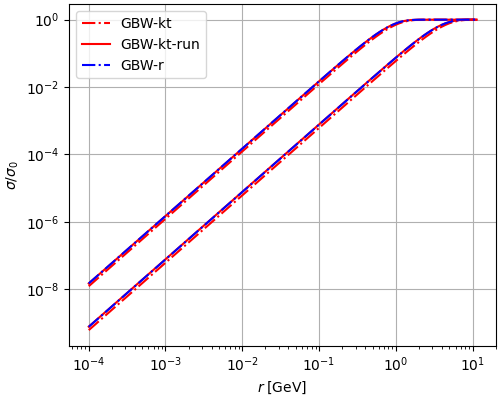
\includegraphics[width=\textwidth]{./plots/GBW-dipole.png}
\end{subfigure}
\begin{subfigure}{0.47\textwidth}
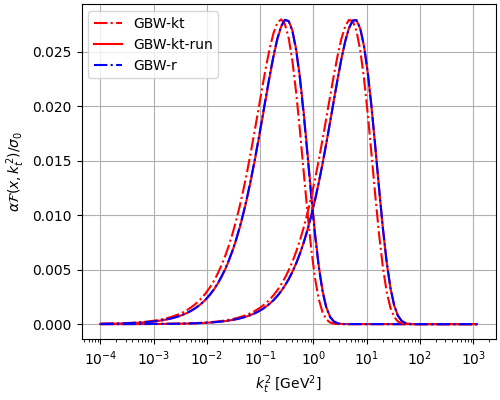
\includegraphics[width=\textwidth]{./plots/GBW-gluon.png}
\end{subfigure}

\begin{subfigure}{0.47\textwidth}
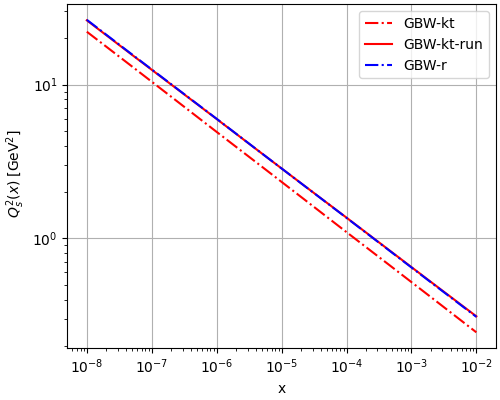
\includegraphics[width=\textwidth]{./plots/GBW-saturation.png}
\end{subfigure}
\caption{The dipole cross section and the dipole gluon density at
$x=10^{-2}, 10^{-6}$, and the saturation scale. 
Note, the dipole cross section and the gluon density are normalized by $\sigma_0^{-1}$.
\comment{The plots do not contain running coupling as the scale depends on $\kappa$ and $m_f$ etc. thus this should be thought of as normalized $\mathcal{F}$, rather than $\alpha\mathcal{F}$.}}
\label{fig:GBW}
\end{figure}


\begin{figure}[t]
	\centering
\begin{subfigure}{0.47\textwidth}
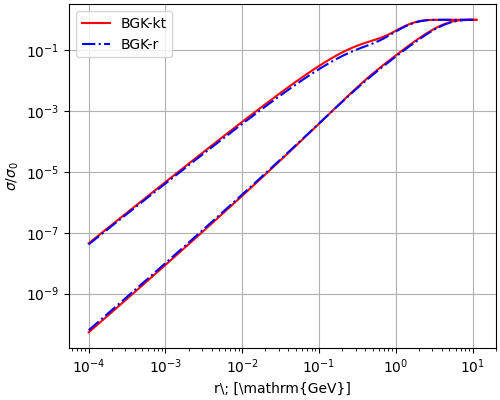
\includegraphics[width=\textwidth]{./plots/BGK-dipole.png}
\end{subfigure}
\begin{subfigure}{0.47\textwidth}
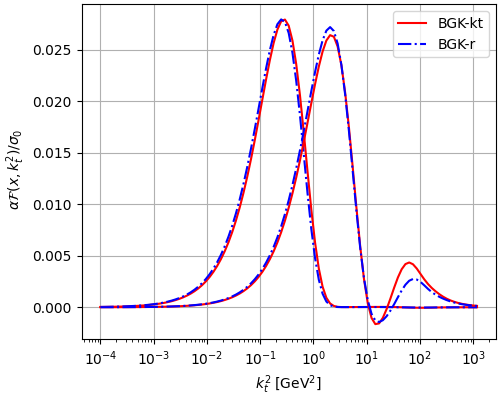
\includegraphics[width=\textwidth]{./plots/BGK-gluon.png}
\end{subfigure}

\begin{subfigure}{0.47\textwidth}
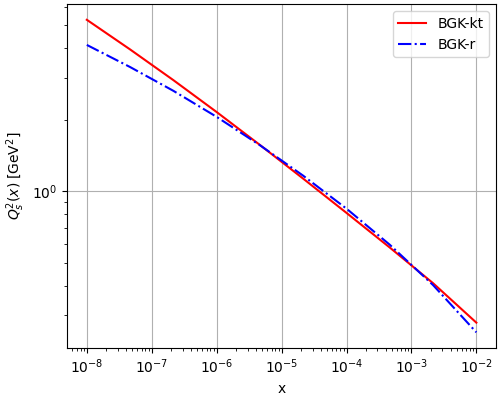
\includegraphics[width=\textwidth]{./plots/BGK-saturation.png}
\end{subfigure}
\caption{The dipole cross section and the dipole gluon density at
$x=10^{-2}, 10^{-6}$, and the saturaton scale. 
Note, the dipole cross section and the gluon density are normalized by $\sigma_0^{-1}$}
\label{fig:BGK}
\end{figure}


\begin{figure}[p]
%\begin{subfigure}{\textwidth}
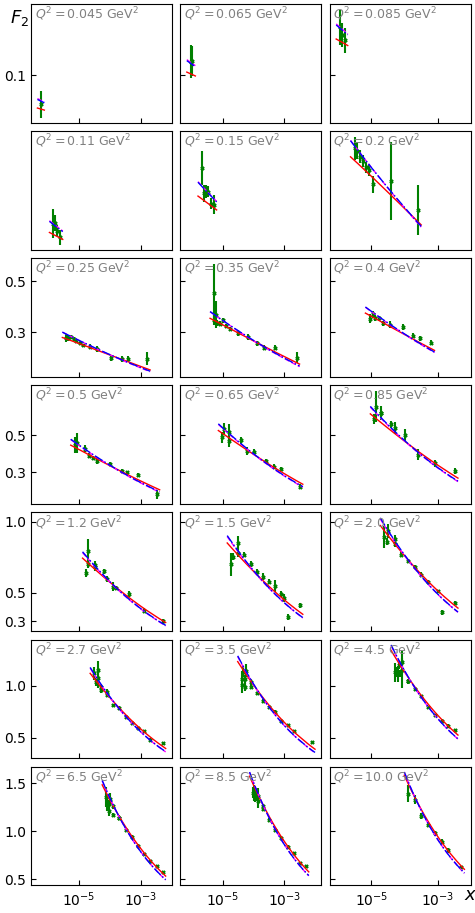
\includegraphics[width=0.49\textwidth]{./plots/Figure_1.png}
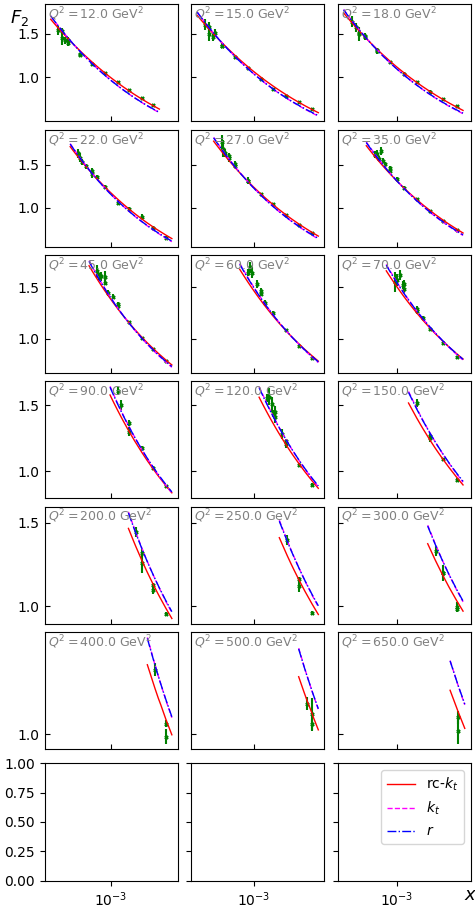
\includegraphics[width=0.49\textwidth]{./plots/Figure_2.png}
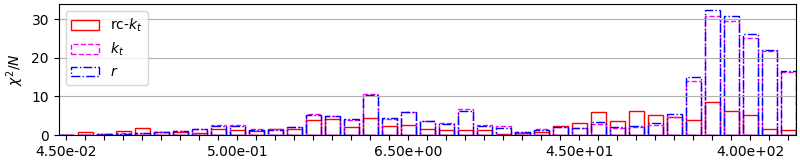
\includegraphics[width=\textwidth]{./plots/Figure_3.png}
\vspace{2mm}
%\end{subfigure}
\caption{Comparison of GBW $F_2$ with HERA data. The histogram shows the $\chi^2$ value per data point in each frame.
 Improvement by the running coupling ($k_t$ run) is clearly visible in the high-$Q^2$region, while the new fit ($k_t$) shows only marginal improvement .  }
\label{fig:GBW-Grid}
\end{figure}
\begin{figure}[p]
%\begin{subfigure}{\textwidth}
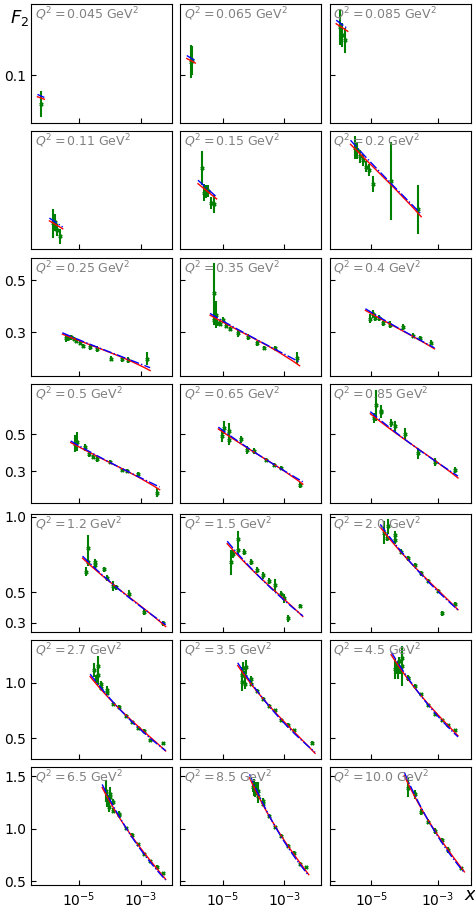
\includegraphics[width=0.49\textwidth]{./plots/Figure_2-1.png}
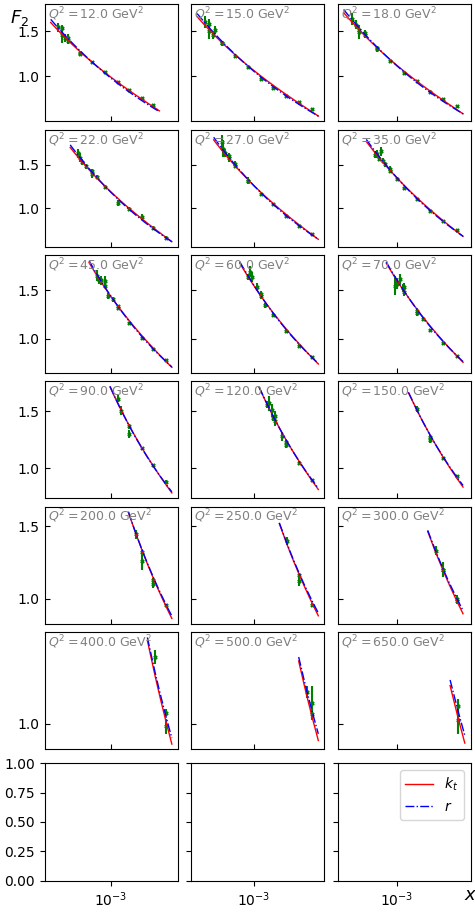
\includegraphics[width=0.49\textwidth]{./plots/Figure_2-2.png}
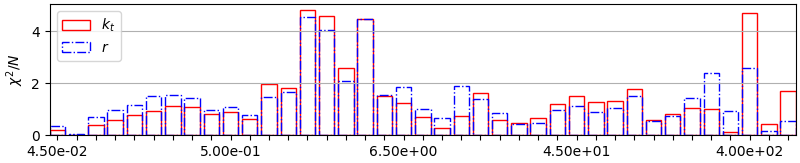
\includegraphics[width=\textwidth]{./plots/Figure_2-3.png}
%\end{subfigure}
\caption{Comparison of BGK $F_2$ with HERA data. The histogram shows the $\chi^2$ value per data point in each frame. While the overall fit quality remain similar, the fit quality in each frame change noticeably. Particularly the $k_t$-formula case ($k_t$) shows better fit in the small-$Q^2$ region.}
\label{fig:BGK-Grid}
\end{figure}

%\begin{figure}[p]
%\center
%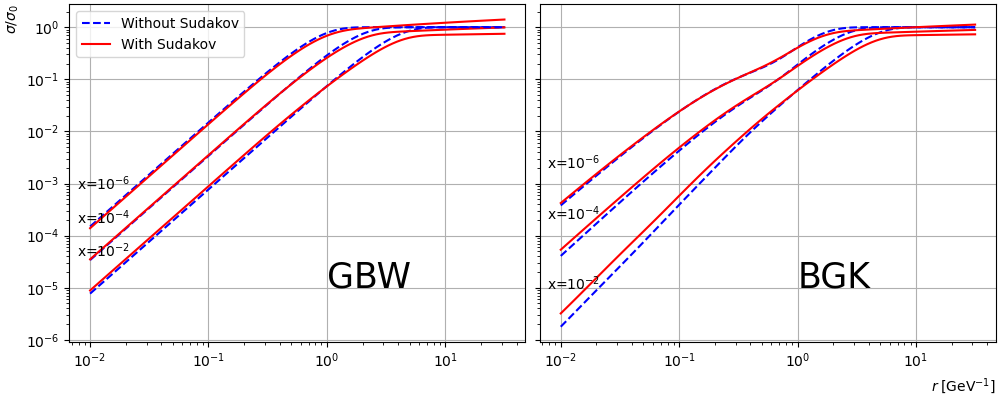
\includegraphics[width=0.9\textwidth]{../plots/dipole-GBW.png}\\
%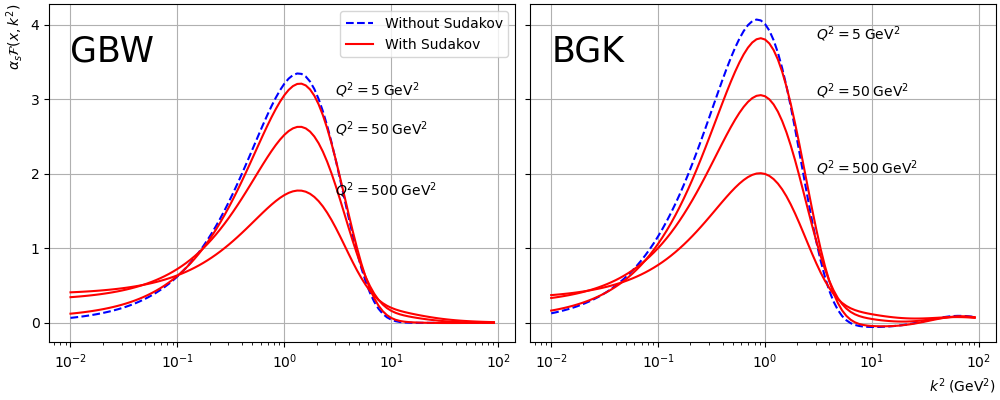
\includegraphics[width=0.9\textwidth]{../plots/gluon-GBW.png}\\
%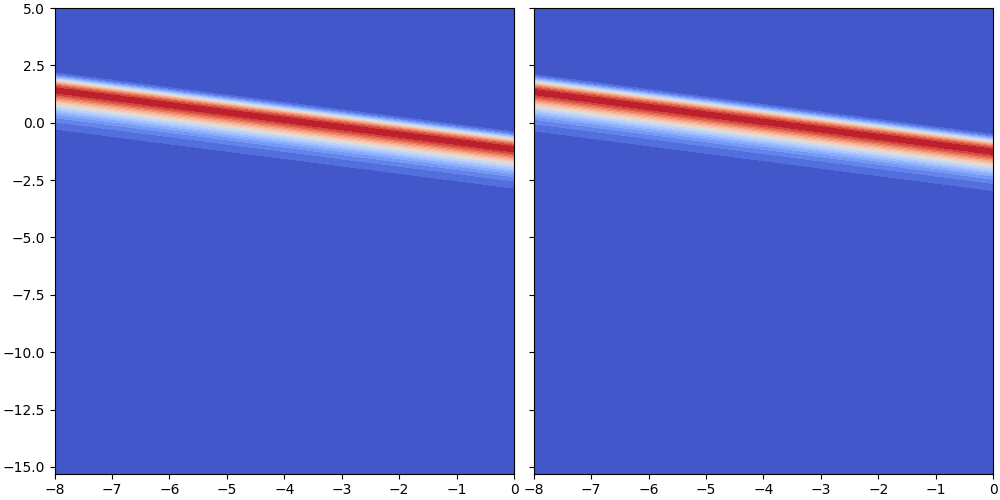
\includegraphics[width=0.9\textwidth]{../plots/gluon-GBW-contour.png}
%\caption{from left: r-BGK, kt-BGK}
%\end{figure}
%\begin{figure}[p]
%\center
%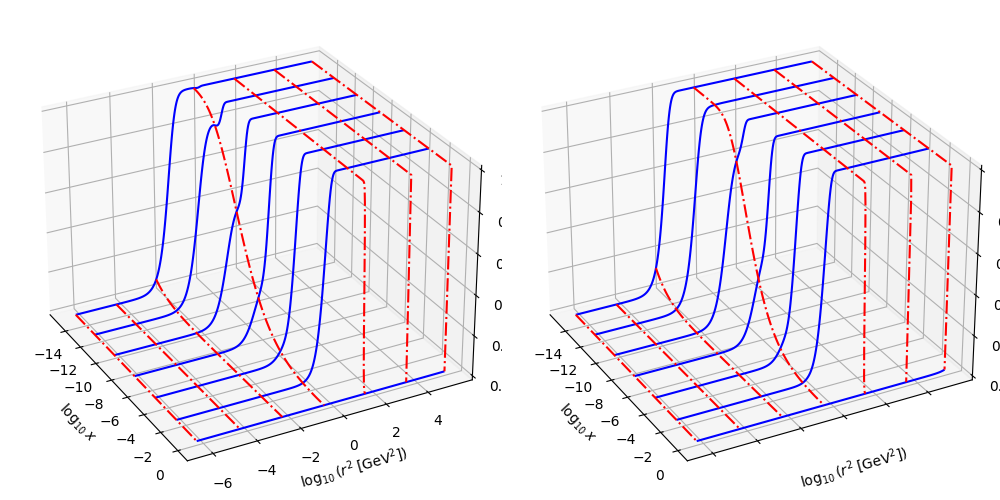
\includegraphics[width=0.9\textwidth]{../plots/dipole-BGK.png}\\
%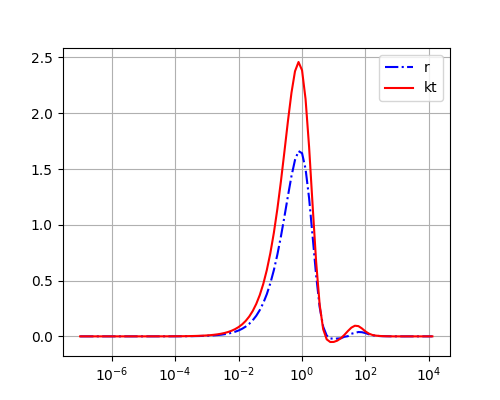
\includegraphics[width=0.9\textwidth]{../plots/gluon-BGK.png}\\
%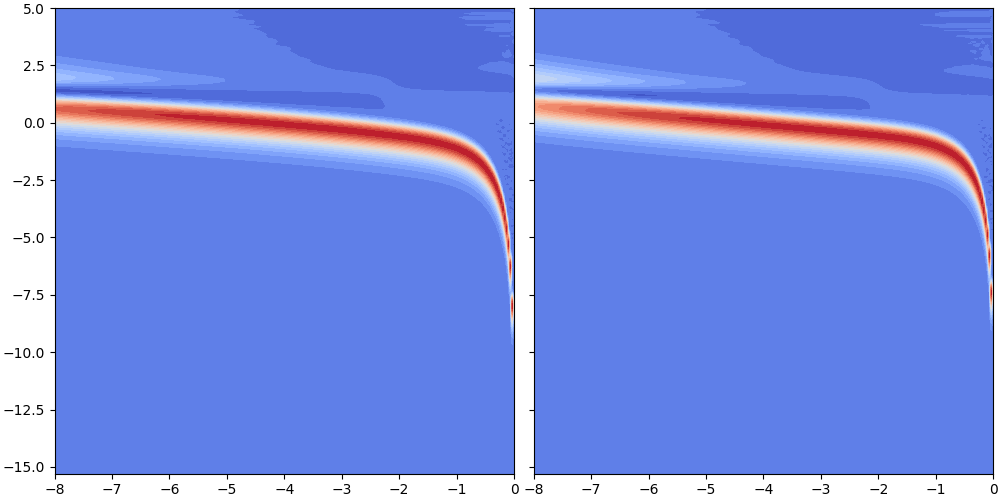
\includegraphics[width=0.9\textwidth]{../plots/gluon-BGK-contour.png}
%\caption{from left: r-BGK, kt-BGK}
%\end{figure}


%%%%%%%%%%%%%%%%%%%%%%%%%%%%%%%%%%%%%%
%
\section{Dijet process at EIC}
\label{Dijet process at EIC}
%
%%%%%%%%%%%%%%%%%%%%%%%%%%%%%%%%%%%%%%%%

\begin{figure}[t]
    \begin{subfigure}{0.5\textwidth}
        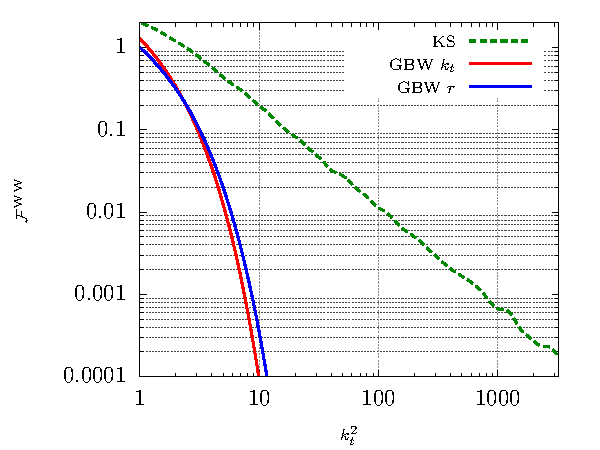
\includegraphics[width=\textwidth]{plots/GBWWW1} 
    \end{subfigure}
    \begin{subfigure}{0.5\textwidth}
        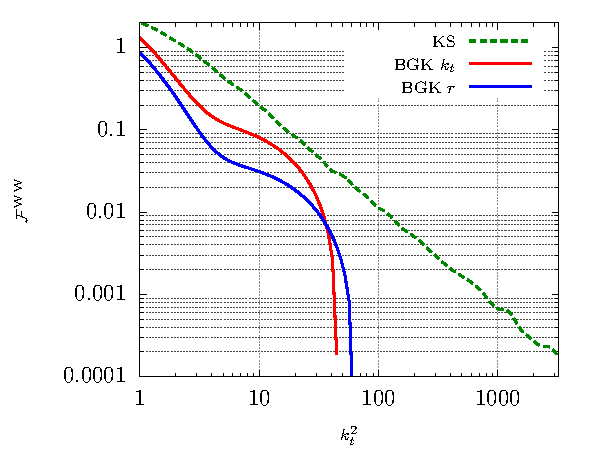
\includegraphics[width=\textwidth]{plots/BGKWW1} 
    \end{subfigure}
    \begin{subfigure}{0.5\textwidth}
        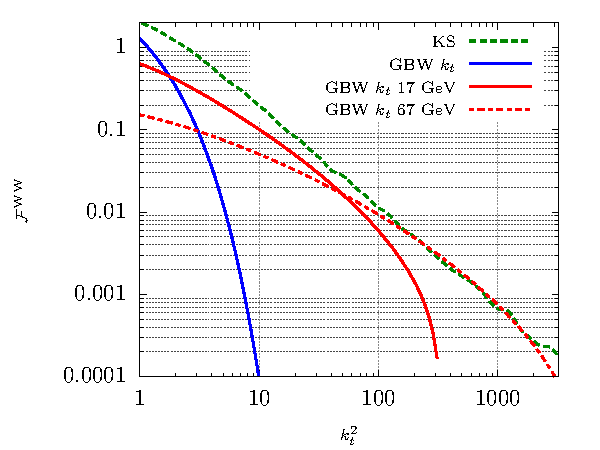
\includegraphics[width=\textwidth]{plots/GBWWW2} 
    \end{subfigure}
    \begin{subfigure}{0.5\textwidth}
        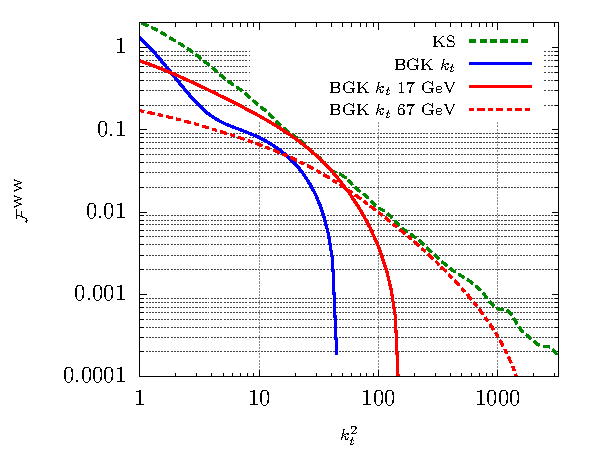
\includegraphics[width=\textwidth]{plots/BGKWW2} 
    \end{subfigure}
    \caption{\footnotesize Weizs\"acker-Williams gluon density at $x=10^{-3}$. Top row: comparison of the dipole-factorization fit and $k_t$-factorization fit results. Bottom row: comparison of the respective models with and without the Sudakov factor, at $\mu=17,\;67 \mathrm{GeV}$. Green dashed line is the KS gluon~\cite{vanHameren:2021sqc}. }
    \label{fig:ww}
\end{figure}
In order to investigate less inclusive processes, we will study the electron-dijet correlation at EIC, following closely the method of Ref.~\cite{vanHameren:2021sqc}. 
The dijet process is known to probe a type of unintegrated gluon density, called Weizs\"acker-Williams gluon density~\cite{Dominguez:2010xd,Dominguez:2011wm,Xiao:2017ggh}.
This UGD, $\fww(x,k^2)$, has an interpretation as a number density of gluons inside a proton~\cite{Dominguez:2010xd,Dominguez:2011wm}. Under the Gaussian approximation and assuming $\theta$-like profile of the proton, one can write~\cite{vanHameren:2016ftb,Xiao:2017ggh,Dominguez:2010xd,Dominguez:2011wm}
\begin{equation}
\fww(x,k^2)= \frac{C_F}{2\pi^3\alpha_s}\int^\infty_0\frac{dr}{r}J_0(r k) \sdpa(x,r),
\end{equation} 	
with the adjoint dipole cross section
\begin{equation}
\sdpa(x,r)=\sigma_0\left( 1-\left(1-\frac{\sdp(x,r)}{\sigma_0}\right)^{C_A/C_F}\right).
\label{eq:ww}
\end{equation}
Resummation of the Sudakov logarithms is achieved by the formula~\cite{Xiao:2017yya}
\begin{equation}
	\fww(x,k^2,\mu^2)= \frac{C_F}{2\pi^3\alpha_s}\int^\infty_0\frac{dr}{r}J_0(r k) e^{-S(r,\mu^2)} \sdpa(x,r),
	\label{eq:ww-sud}
\end{equation}
where, we use the Sudakov form factor~\cite{Mueller:2013wwa,Xiao:2017yya},
\begin{equation}
	S(r,\mu^2)=\frac{\alpha_s N_c}{4\pi}\ln^2\left(\frac{\mu^2r^2}{4e^{-2\gamma_E}}\right),
\end{equation}
in which $\gamma_E$ is the Euler-Mascheroni constant, and we use $\alpha_s=0.2$. 
 

  
The present study is carried out in the framework of the small-$x$-Improved Transverse-Momentum-Dependent (ITMD) factorization~\cite{Kotko:2015ura,vanHameren:2016ftb}.
The ITMD factorization is implemented in the program KaTie~\cite{vanHameren:2016kkz}, which we will use to compute the cross section. Important points of the formalism are the following. Firstly, it extends applicability of TMD to the large-$k_t$ region. Thus it recovers the $k_t$-factorization if saturation effects are neglected\comment{what does this mean exactly? why are we using saturation model?}. Secondly, it is equivalent to CGC, where $(Q_s/k_t)^n$ and $(k_t/P_t)^n$ are resummed, except for lacking multipartonic interaction~(genuine twist)~\cite{vanHameren:2016kkz,Altinoluk:2019fui}. It was discussed in Ref.~\cite{vanHameren:2021sqc}, that with the above points and the fact that genuine twists are suppressed when transverse momenta are large \comment{Also, $Q$ but as it was also said, that Q is low here(p.5,\cite{vanHameren:2021sqc}. )  Also it was mentioned the cut on $p_T$ is selected for this. I assume it is $p_{1T}, p_{2T}$ that are relevant?}, ITMD is suitable for studying dijets.

Following Ref.~\cite{vanHameren:2021sqc}, we study the azimuthal correlations of jets and the final state electron in DIS ($e+p\rightarrow e+J_1+J_2+X$), where it was argued that this observable is sensitive to the soft emissions and the saturation effects. 
The kinematical cuts suggested in Ref.~\cite{vanHameren:2021sqc} were
\begin{align*}
	E_e&=15\GeV& E_p&=135\GeV& Q^2&>1\GeV^2\\
	0.1<&\nu<0.85&\Delta R_{\mathrm{Breit}}&<1&p^{\mathrm{Breit}}_{1,2\,T}&>3\GeV\\
	&&-4<&y_{1,2\,\mathrm{lab}}<-1.&&
\end{align*}

Grids of the Weizs\"acker-Williams gluon density were produced by evaluating Eqs.~(\ref{eq:ww}) and~(\ref{eq:ww-sud}).
The gluon density at $x=10^{-3}$ is plotted in Fig.~\ref{fig:ww} with hard-scale-independent KS gluon~\cite{vanHameren:2021sqc}. Clearly, the GBW and BGK models falls much more quickly than the KS gluon density. In general, expected behaviour in the large-$k_t$ region is $\sim k_t^{-2}$~\cite{Dominguez:2010xd,Dominguez:2011wm}, while GBW behaves like $\sim e^{-k_t^2}$.
As in Ref.~\cite{vanHameren:2021sqc}, the Sudakov factor enhances in the small-$k_t$ region and suppresses in the large-$k_t$ region. In other words it broadens the distribution. In comparison to the result of Ref.~\cite{vanHameren:2021sqc}, the effect of broadening by the Sudakov is significantly more pronounced in the case of the GBW and BGK models. The hard-scale-dependent GBW and BGK models, as a consequence, become closer to the KS gluon (\textit{cf.} Fig.~2 of Ref.~\cite{vanHameren:2021sqc}).  

Figs.~\ref{fig:je-breit} and~\ref{fig:je-lab} correspond to Fig.~4 in Ref.~\cite{vanHameren:2021sqc} ($e$-jets azimuthal correlation). 
In the top row of Fig.~\ref{fig:je-breit}, we see, for both the GBW and BGK models, better agreements of results with the KS for the new $k_t$-factorization fits. However the overall normalization of the gluon density depends on the coupling $\alpha_s$, which we assumed to be 0.2. In the middle and the bottom row, it shows the effects of the Sudakov form factor, which qualitatively agrees with that of Ref.~\cite{vanHameren:2021sqc}, by lowering the cross section.
Fig.~\ref{fig:je-lab} shows the $e$-jets correlation in the lab frame. Here, the difference between KS and GBW and BGK are more prominent. %Unlike in the previous plots, the new fits in the $k_t$-factorization shows only limited improvement.
The effects of the Sudakov factor is similar to those in Ref.~\cite{vanHameren:2021sqc} at relatively high $\Delta \phi$, while at smaller $\Delta \phi$ region the effect is reversed (i.e. The cross sections were slightly lowered in Ref.~\cite{vanHameren:2021sqc}, while here, they are significantly increased). \\
\comment{regarding this differences between Breit and lab frames, what does "\dots since it (breit) suppresses the LO contributions, i.e. process dominated by a quark jet." mean?}

\begin{figure}[p]
	\begin{subfigure}{0.5\textwidth}
	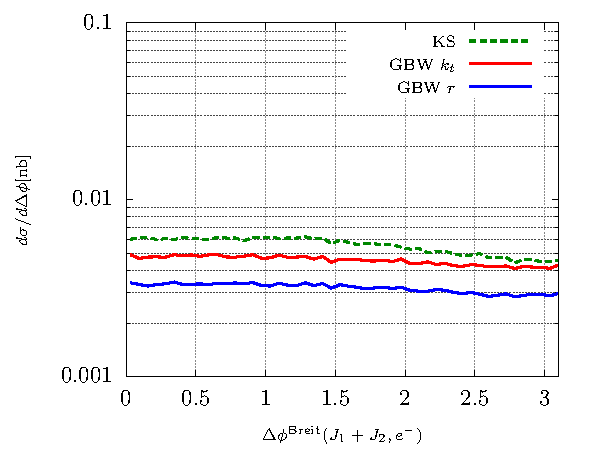
\includegraphics[width=\textwidth]{plots/plotGBW1} 
	\end{subfigure}
	\begin{subfigure}{0.5\textwidth}
	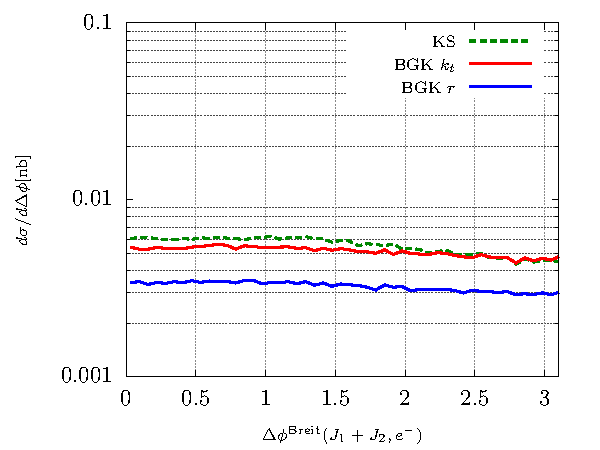
\includegraphics[width=\textwidth]{plots/plotBGK1} 
	\end{subfigure}
%	\caption{ }
%\end{figure}
%\begin{figure}[t]
	\begin{subfigure}{0.5\textwidth}
	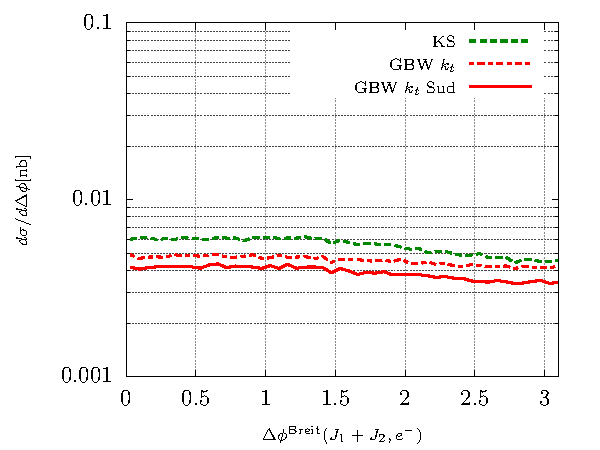
\includegraphics[width=\textwidth]{plots/plotGBW2}
	\end{subfigure}
	\begin{subfigure}{0.5\textwidth}
	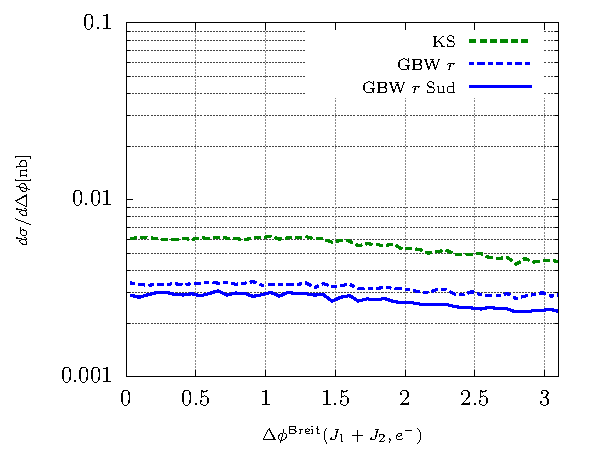
\includegraphics[width=\textwidth]{plots/plotGBW3}
	\end{subfigure}
	\begin{subfigure}{0.5\textwidth}
	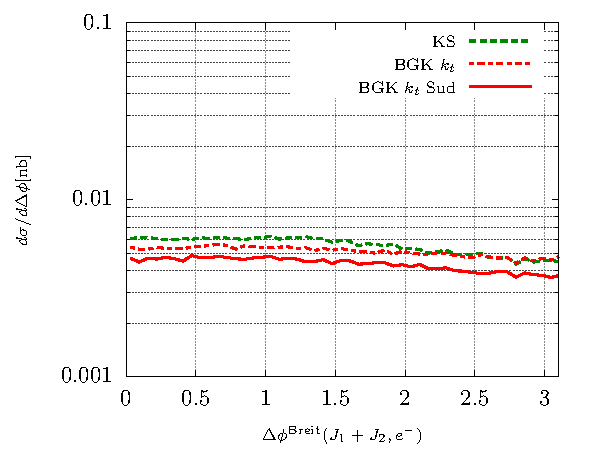
\includegraphics[width=\textwidth]{plots/plotBGK2}
	\end{subfigure}
	\begin{subfigure}{0.5\textwidth}
	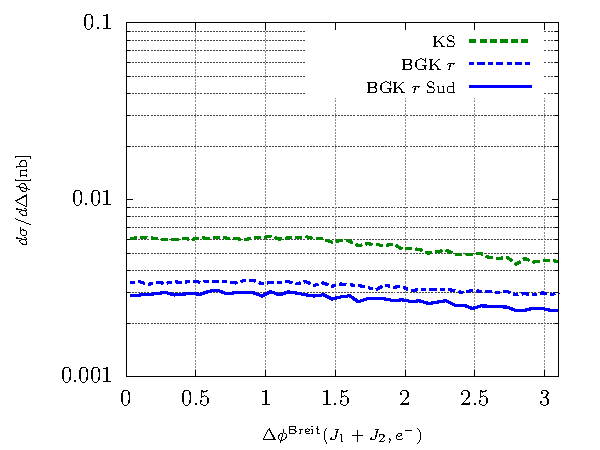
\includegraphics[width=\textwidth]{plots/plotBGK3}
	\end{subfigure}
	\caption{\footnotesize Azimuthal correlation of the jets and the scattered electron in the Breit frame. Top: Comparison of dipole-factorization fit and $k_t$-factorization fit. Middle \& Bottom: Effect of the Sudakov form factor.   Green dashed line is the KS gluon~\cite{vanHameren:2021sqc}.}
	\label{fig:je-breit}
\end{figure}

\begin{figure}[p]
	\begin{subfigure}{0.5\textwidth}
		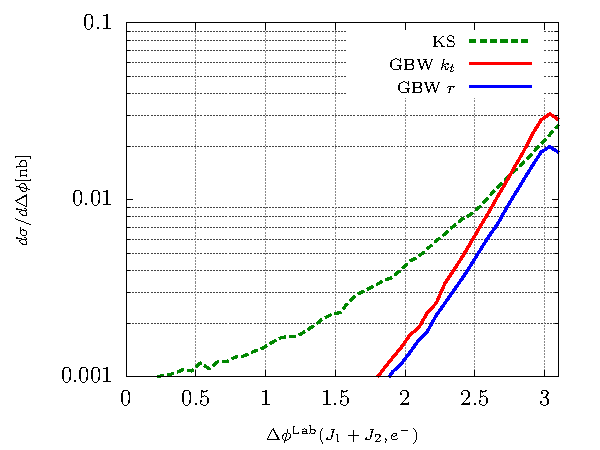
\includegraphics[width=\textwidth]{plots/plotGBW1Lab} 
	\end{subfigure}
	\begin{subfigure}{0.5\textwidth}
		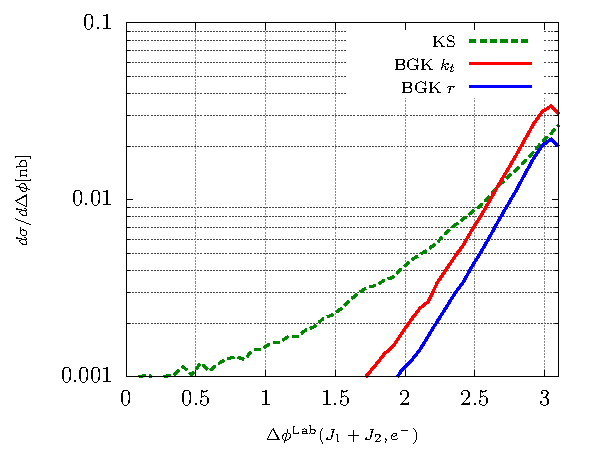
\includegraphics[width=\textwidth]{plots/plotBGK1Lab} 
	\end{subfigure}

	\begin{subfigure}{0.5\textwidth}
		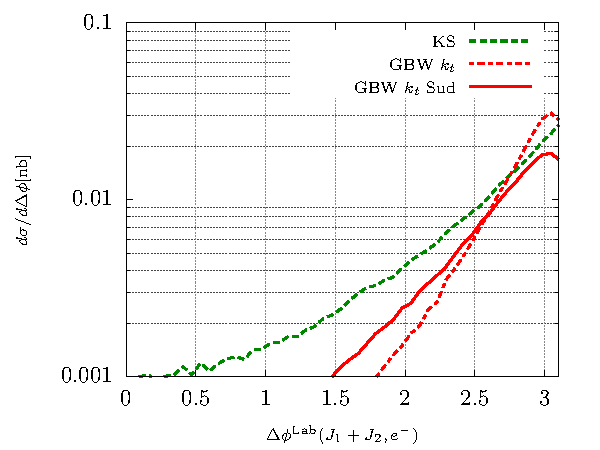
\includegraphics[width=\textwidth]{plots/plotGBW2Lab}
	\end{subfigure}
	\begin{subfigure}{0.5\textwidth}
		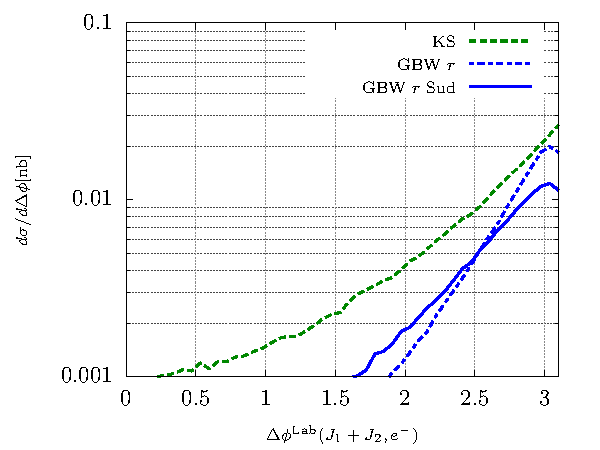
\includegraphics[width=\textwidth]{plots/plotGBW3Lab}
	\end{subfigure}

	\begin{subfigure}{0.5\textwidth}
		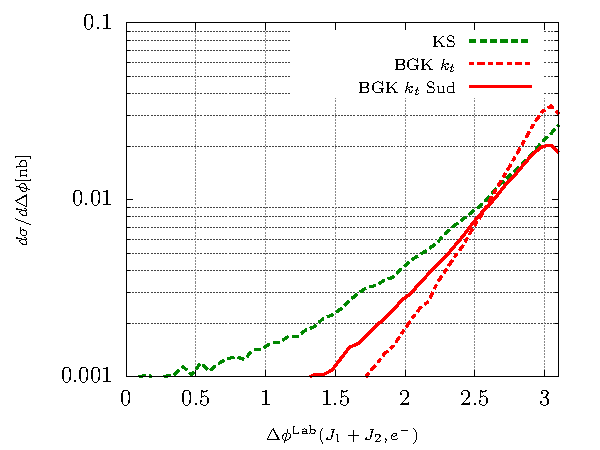
\includegraphics[width=\textwidth]{plots/plotBGK2Lab}
	\end{subfigure}
	\begin{subfigure}{0.5\textwidth}
		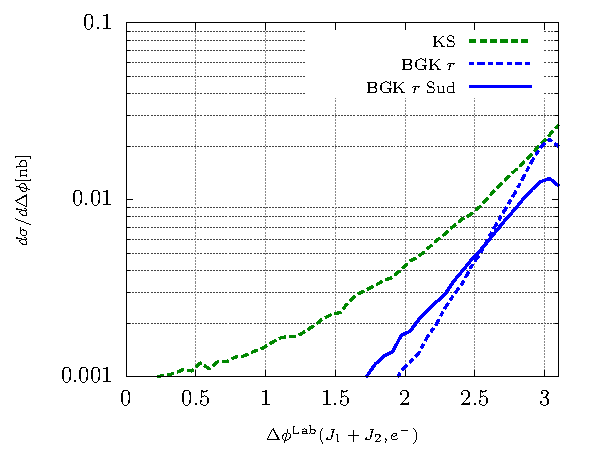
\includegraphics[width=\textwidth]{plots/plotBGK3Lab}
	\end{subfigure}
\caption{\footnotesize Azimuthal correlation of the jets and the scattered electron in the lab frame. Top: Comparison of dipole-factorization fit and $k_t$-factorization fit. Middle \& Bottom: Effect of the Sudakov form factor.  Green dashed line is the KS gluon~\cite{vanHameren:2021sqc}.}
\label{fig:je-lab}
\end{figure}

Finally, Fig.~\ref{fig:jj-breit} shows the jet correlations in the Breit frame. Again, the GBW and BGK models show considerable deviation from the KS gluon. Similarly to the previous plots, the Sudakov factor affects the models differently from the KS gluon in Ref.~\cite{vanHameren:2021sqc}.
The effect enhances the cross section considerably in the small-$\Delta\phi$ region, making it closer to KS gluon result.
The results shown in Figs.~\ref{fig:je-lab} and~\ref{fig:jj-breit} are natural as back-to-back configuration in the respective observable corresponds to the small-$k_t$ region of gluon densities, and as it can be seen clearly in Fig.~\ref{fig:ww}, the GBW and BGK gluons do not fare well in the large-$k_t$ region. 
That is to say that the enhancement in the small-$\Delta\phi$ region is a direct consequence of the broadening by the Sudakov factor. 

\begin{figure}[p]
	\begin{subfigure}{0.5\textwidth}
		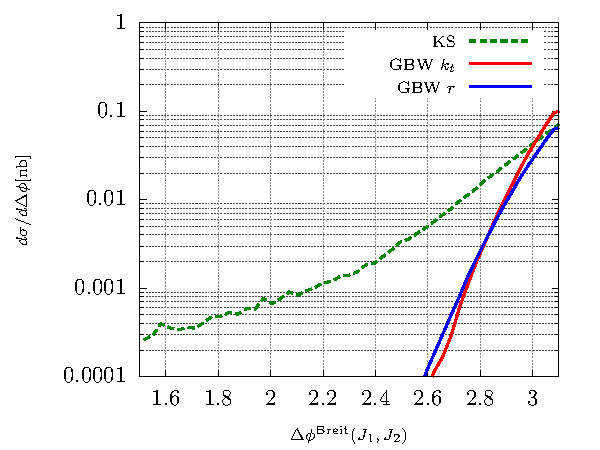
\includegraphics[width=\textwidth]{plots/plotGBW1Jets} 
	\end{subfigure}
	\begin{subfigure}{0.5\textwidth}
		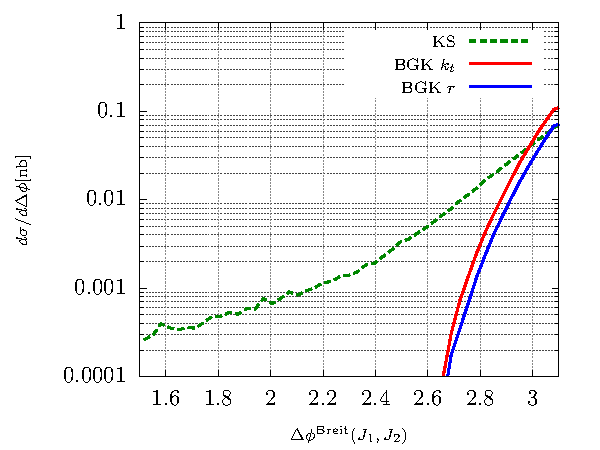
\includegraphics[width=\textwidth]{plots/plotBGK1Jets} 
	\end{subfigure}

	\begin{subfigure}{0.5\textwidth}
		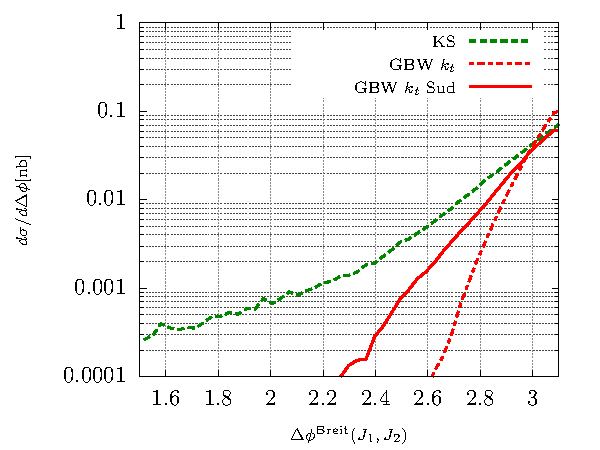
\includegraphics[width=\textwidth]{plots/plotGBW2Jets}
	\end{subfigure}
	\begin{subfigure}{0.5\textwidth}
		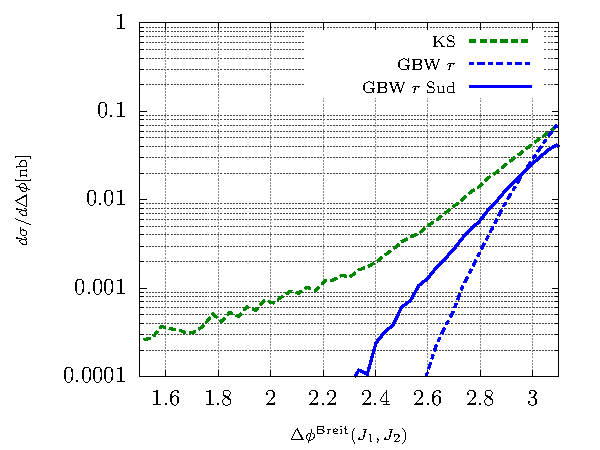
\includegraphics[width=\textwidth]{plots/plotGBW3Jets}
	\end{subfigure}

	\begin{subfigure}{0.5\textwidth}
		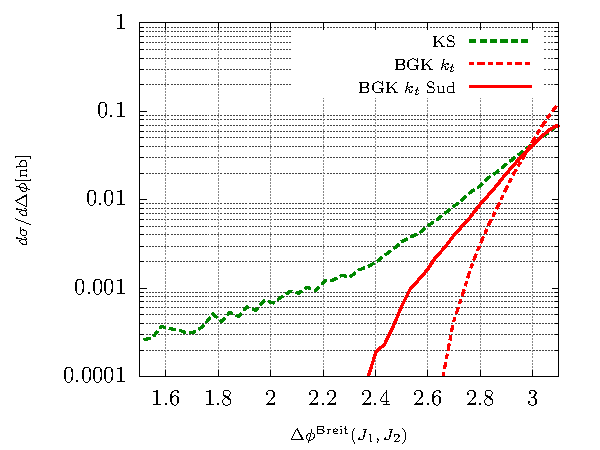
\includegraphics[width=\textwidth]{plots/plotBGK2Jets}
	\end{subfigure}
	\begin{subfigure}{0.5\textwidth}
		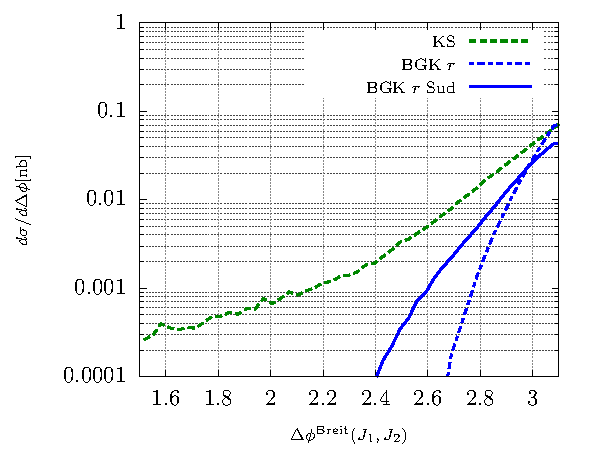
\includegraphics[width=\textwidth]{plots/plotBGK3Jets}
	\end{subfigure}
\caption{\footnotesize Azimuthal correlation of the jets in the Breit frame. Top: Comparison of dipole-factorization fit and $k_t$-factorization fit. Middle \& Bottom: Effect of the Sudakov form factor. Green dashed line is the KS gluon~\cite{vanHameren:2021sqc}. }
\label{fig:jj-breit}
\end{figure}

\section{Summary}
We have fitted the Golec-Biernat--W\"usthoff~(GBW)\cite{Golec-Biernat:1998zce} and Bartels--Golec-Biernat--Kowalski~(BGK)~\cite{Bartels:2002cj} models to the HERA data~\cite{Abt:2017nkc} in the context of the $k_t$-factorization of $F_2$.  The main difference between the $k_t$- and dipole-factorizations is an argument of the gluon, that is, $x/z$ being replaced by $x(1+4m_f^2/Q^2)$ in the dipole-factorization. It was discussed that massive light quarks used in Ref.~\cite{Golec-Biernat:1998zce} partially simulates the factor $1/z$, and the fit result indicates such effect as expected. It is quite remarkable that with such simplicity, the dipole-factorization can reproduce the result of the $k_t$-factorization formula well. Only major difference is in the normalization parameter $\sigma_0$ which increases significantly for the $k_t$-factorization case. It was also observed that the explicit inclusion of the running coupling has significant effect in the fit quality particularly in the large-$Q^2$ region where the GBW model performs poorly. 
We have applied the new result for the prediction of the dijet process in DIS at EIC. Additionally, effects of the Sudakov form factor was investigated. Results of the $e$-jets correlation in the Breit frame agree qualitatively to that of Ref.~\cite{vanHameren:2021sqc}. Other results, namely the $e$-jets in the lab frame and the jet-jet correlation in the Breit frame, show considerable effects of the Sudakov form factor which broaden the gluon density.  

\section*{Acknowledment}


%%%%%%%%%%%%%%%%%%%%%%%%%%%%%%%%%%%%%%%%%%%
\clearpage
%\bibliography{draft}
\printbibliography

%\begin{thebibliography}{10}
%\bibliographystyle{unsrt} 

%%\cite{vanHameren:2021sqc}
\bibitem{vanHameren:2021sqc}
A.~van Hameren, P.~Kotko, K.~Kutak, S.~Sapeta and E.~\.Zar\'ow,
%``Probing gluon number density with electron-dijet correlations at EIC,''
Eur. Phys. J. C \textbf{81} (2021) no.8, 741
doi:10.1140/epjc/s10052-021-09529-3
[arXiv:2106.13964 [hep-ph]].
%12 citations counted in INSPIRE as of 18 Apr 2023

%\cite{Kovchegov:2012mbw}
\bibitem{Kovchegov:2012mbw}
Y.~V.~Kovchegov and E.~Levin,
%``Quantum Chromodynamics at High Energy,''
Camb. Monogr. Part. Phys. Nucl. Phys. Cosmol. \textbf{33} (2012), 1-350
Oxford University Press, 2013,
ISBN 978-1-00-929144-6, 978-1-00-929141-5, 978-1-00-929142-2, 978-0-521-11257-4, 978-1-139-55768-9
doi:10.1017/9781009291446
%266 citations counted in INSPIRE as of 14 Apr 2023

%\cite{Dominguez:2010xd}
\bibitem{Dominguez:2010xd}
F.~Dominguez, B.~W.~Xiao and F.~Yuan,
%``$k_t$-factorization for Hard Processes in Nuclei,''
Phys. Rev. Lett. \textbf{106} (2011), 022301
doi:10.1103/PhysRevLett.106.022301
[arXiv:1009.2141 [hep-ph]].
%158 citations counted in INSPIRE as of 11 Apr 2023

%\cite{Dominguez:2011wm}
\bibitem{Dominguez:2011wm}
F.~Dominguez, C.~Marquet, B.~W.~Xiao and F.~Yuan,
%``Universality of Unintegrated Gluon Distributions at small x,''
Phys. Rev. D \textbf{83} (2011), 105005
doi:10.1103/PhysRevD.83.105005
[arXiv:1101.0715 [hep-ph]].
%381 citations counted in INSPIRE as of 11 Apr 2023

%\cite{Xiao:2017yya}
\bibitem{Xiao:2017yya}
B.~W.~Xiao, F.~Yuan and J.~Zhou,
%``Transverse Momentum Dependent Parton Distributions at Small-x,''
Nucl. Phys. B \textbf{921} (2017), 104-126
doi:10.1016/j.nuclphysb.2017.05.012
[arXiv:1703.06163 [hep-ph]].
%39 citations counted in INSPIRE as of 11 Apr 2023

%\cite{Balitsky:1978ic}
\bibitem{Balitsky:1978ic}
I.~I.~Balitsky and L.~N.~Lipatov,
%``The Pomeranchuk Singularity in Quantum Chromodynamics,''
Sov. J. Nucl. Phys. \textbf{28} (1978), 822-829
%3937 citations counted in INSPIRE as of 19 Apr 2023

%\cite{Kuraev:1977fs}
\bibitem{Kuraev:1977fs}
E.~A.~Kuraev, L.~N.~Lipatov and V.~S.~Fadin,
%``The Pomeranchuk Singularity in Nonabelian Gauge Theories,''
Sov. Phys. JETP \textbf{45} (1977), 199-204
%3562 citations counted in INSPIRE as of 18 Apr 2023

%\cite{Barone:1993sy}
\bibitem{Barone:1993sy}
V.~Barone, M.~Genovese, N.~N.~Nikolaev, E.~Predazzi and B.~G.~Zakharov,
%``Unitarization of structure functions at large 1/x,''
Phys. Lett. B \textbf{326} (1994), 161-167
doi:10.1016/0370-2693(94)91208-4
[arXiv:hep-ph/9307248 [hep-ph]].
%41 citations counted in INSPIRE as of 15 Mar 2023

%\cite{Balitsky:1995ub}
\bibitem{Balitsky:1995ub}
I.~Balitsky,
%``Operator expansion for high-energy scattering,''
Nucl. Phys. B \textbf{463} (1996), 99-160
doi:10.1016/0550-3213(95)00638-9
[arXiv:hep-ph/9509348 [hep-ph]].
%1819 citations counted in INSPIRE as of 14 Apr 2023

%\cite{Kovchegov:1999yj}
\bibitem{Kovchegov:1999yj}
Y.~V.~Kovchegov,
%``Small x F(2) structure function of a nucleus including multiple pomeron exchanges,''
Phys. Rev. D \textbf{60} (1999), 034008
doi:10.1103/PhysRevD.60.034008
[arXiv:hep-ph/9901281 [hep-ph]].
%1618 citations counted in INSPIRE as of 14 Apr 2023

%\cite{Golec-Biernat:1998zce}
\bibitem{Golec-Biernat:1998zce}
K.~J.~Golec-Biernat and M.~Wusthoff,
%``Saturation effects in deep inelastic scattering at low Q**2 and its implications on diffraction,''
Phys. Rev. D \textbf{59} (1998), 014017
doi:10.1103/PhysRevD.59.014017
[arXiv:hep-ph/9807513 [hep-ph]].
%1424 citations counted in INSPIRE as of 13 Apr 2023

%\cite{Kowalski:2003hm}
\bibitem{Kowalski:2003hm}
H.~Kowalski and D.~Teaney,
%``An Impact parameter dipole saturation model,''
Phys. Rev. D \textbf{68} (2003), 114005
doi:10.1103/PhysRevD.68.114005
[arXiv:hep-ph/0304189 [hep-ph]].
%515 citations counted in INSPIRE as of 17 Apr 2023

%\cite{McLerran:1993ni}
\bibitem{McLerran:1993ni}
L.~D.~McLerran and R.~Venugopalan,
%``Computing quark and gluon distribution functions for very large nuclei,''
Phys. Rev. D \textbf{49} (1994), 2233-2241
doi:10.1103/PhysRevD.49.2233
[arXiv:hep-ph/9309289 [hep-ph]].
%2221 citations counted in INSPIRE as of 17 Apr 2023

%\cite{Forshaw:1999uf}
\bibitem{Forshaw:1999uf}
J.~R.~Forshaw, G.~Kerley and G.~Shaw,
%``Extracting the dipole cross-section from photoproduction and electroproduction total cross-section data,''
Phys. Rev. D \textbf{60} (1999), 074012
doi:10.1103/PhysRevD.60.074012
[arXiv:hep-ph/9903341 [hep-ph]].
%135 citations counted in INSPIRE as of 01 Apr 2023

%\cite{Iancu:2003ge}
\bibitem{Iancu:2003ge}
E.~Iancu, K.~Itakura and S.~Munier,
%``Saturation and BFKL dynamics in the HERA data at small x,''
Phys. Lett. B \textbf{590} (2004), 199-208
doi:10.1016/j.physletb.2004.02.040
[arXiv:hep-ph/0310338 [hep-ph]].
%497 citations counted in INSPIRE as of 15 Mar 2023

%\cite{Bartels:2002cj}
\bibitem{Bartels:2002cj}
J.~Bartels, K.~J.~Golec-Biernat and H.~Kowalski,
%``A modification of the saturation model: DGLAP evolution,''
Phys. Rev. D \textbf{66} (2002), 014001
doi:10.1103/PhysRevD.66.014001
[arXiv:hep-ph/0203258 [hep-ph]].
%441 citations counted in INSPIRE as of 11 Apr 2023

%\cite{Golec-Biernat:1999qor}
\bibitem{Golec-Biernat:1999qor}
K.~J.~Golec-Biernat and M.~Wusthoff,
%``Saturation in diffractive deep inelastic scattering,''
Phys. Rev. D \textbf{60} (1999), 114023
doi:10.1103/PhysRevD.60.114023
[arXiv:hep-ph/9903358 [hep-ph]].
%928 citations counted in INSPIRE as of 15 Mar 2023

%\cite{Kimber:2001uaa}
\bibitem{Kimber:2001uaa}
M.~Kimber,
%``Unintegrated parton distributions,''
%1 citations counted in INSPIRE as of 15 Mar 2023

%\cite{Kwiecinski:1997ee}
\bibitem{Kwiecinski:1997ee}
J.~Kwiecinski, A.~D.~Martin and A.~M.~Stasto,
%``A Unified BFKL and GLAP description of F2 data,''
Phys. Rev. D \textbf{56} (1997), 3991-4006
doi:10.1103/PhysRevD.56.3991
[arXiv:hep-ph/9703445 [hep-ph]].
%258 citations counted in INSPIRE as of 15 Mar 2023

%\cite{Luszczak:2022fkf}
\bibitem{Luszczak:2022fkf}
A.~\L{}uszczak, M.~\L{}uszczak and W.~Sch\"afer,
%``Unintegrated gluon distributions from the color dipole cross section in the BGK saturation model,''
Phys. Lett. B \textbf{835} (2022), 137582
doi:10.1016/j.physletb.2022.137582
[arXiv:2210.02877 [hep-ph]].
%3 citations counted in INSPIRE as of 15 Mar 2023

%\cite{Abt:2017nkc}
\bibitem{Abt:2017nkc}
I.~Abt, A.~M.~Cooper-Sarkar, B.~Foster, V.~Myronenko, K.~Wichmann and M.~Wing,
%``Investigation into the limits of perturbation theory at low $Q^2$ using HERA deep inelastic scattering data,''
Phys. Rev. D \textbf{96} (2017) no.1, 014001
doi:10.1103/PhysRevD.96.014001
[arXiv:1704.03187 [hep-ex]].
%14 citations counted in INSPIRE as of 15 Mar 2023

%\cite{Kolbig:1972zz}
\bibitem{Kolbig:1972zz}
K.~S.~Kolbig,
%``PROGRAMS FOR COMPUTING THE LOGARITHM OF THE GAMMA FUNCTION AND THE DIGAMMA FUNCTION FOR COMPLEX ARGUMENT,''
CERN-DD-72-7.
%0 citations counted in INSPIRE as of 15 Mar 2023

%\cite{Hahn:2004fe}
\bibitem{Hahn:2004fe}
T.~Hahn,
%``CUBA: A Library for multidimensional numerical integration,''
Comput. Phys. Commun. \textbf{168} (2005), 78-95
doi:10.1016/j.cpc.2005.01.010
[arXiv:hep-ph/0404043 [hep-ph]].
%718 citations counted in INSPIRE as of 19 Apr 2023

%\cite{Brun:1997pa}
\bibitem{Brun:1997pa}
R.~Brun and F.~Rademakers,
%``ROOT: An object oriented data analysis framework,''
Nucl. Instrum. Meth. A \textbf{389} (1997), 81-86
doi:10.1016/S0168-9002(97)00048-X
%3299 citations counted in INSPIRE as of 18 Apr 2023

%\cite{Goda:2022wsc}
\bibitem{Goda:2022wsc}
T.~Goda, K.~Kutak and S.~Sapeta,
%``Sudakov effects and the dipole amplitude,''
Nucl. Phys. B \textbf{990} (2023), 116155
doi:10.1016/j.nuclphysb.2023.116155
[arXiv:2210.16084 [hep-ph]].
%1 citations counted in INSPIRE as of 06 Apr 2023

%\cite{James:2004xla}
\bibitem{James:2004xla}
F.~James and M.~Winkler,
%``MINUIT User's Guide,''
%7 citations counted in INSPIRE as of 15 Mar 2023

%\cite{Albacete:2004gw}
\bibitem{Albacete:2004gw}
J.~L.~Albacete, N.~Armesto, J.~G.~Milhano, C.~A.~Salgado and U.~A.~Wiedemann,
%``Numerical analysis of the Balitsky-Kovchegov equation with running coupling: Dependence of the saturation scale on nuclear size and rapidity,''
Phys. Rev. D \textbf{71} (2005), 014003
doi:10.1103/PhysRevD.71.014003
[arXiv:hep-ph/0408216 [hep-ph]].
%143 citations counted in INSPIRE as of 15 Mar 2023

%\cite{Albacete:2007yr}
\bibitem{Albacete:2007yr}
J.~L.~Albacete and Y.~V.~Kovchegov,
%``Solving high energy evolution equation including running coupling corrections,''
Phys. Rev. D \textbf{75} (2007), 125021
doi:10.1103/PhysRevD.75.125021
[arXiv:0704.0612 [hep-ph]].
%219 citations counted in INSPIRE as of 15 Mar 2023

%\cite{Albacete:2010sy}
\bibitem{Albacete:2010sy}
J.~L.~Albacete, N.~Armesto, J.~G.~Milhano, P.~Quiroga-Arias and C.~A.~Salgado,
%``AAMQS: A non-linear QCD analysis of new HERA data at small-x including heavy quarks,''
Eur. Phys. J. C \textbf{71} (2011), 1705
doi:10.1140/epjc/s10052-011-1705-3
[arXiv:1012.4408 [hep-ph]].
%273 citations counted in INSPIRE as of 30 Mar 2023

%\cite{Kutak:2004ym}
\bibitem{Kutak:2004ym}
K.~Kutak and A.~M.~Stasto,
%``Unintegrated gluon distribution from modified BK equation,''
Eur. Phys. J. C \textbf{41} (2005), 343-351
doi:10.1140/epjc/s2005-02223-0
[arXiv:hep-ph/0408117 [hep-ph]].
%112 citations counted in INSPIRE as of 15 Mar 2023

%\cite{Xiao:2017ggh}
\bibitem{Xiao:2017ggh}
B.~W.~Xiao,
%``Low-$x$ Physics in $pA$ Collisions and at the EIC,''
Nucl. Phys. A \textbf{967} (2017), 257-264
doi:10.1016/j.nuclphysa.2017.05.024
[arXiv:1704.03662 [nucl-th]].
%1 citations counted in INSPIRE as of 15 Mar 2023

%\cite{vanHameren:2016ftb}
\bibitem{vanHameren:2016ftb}
A.~van Hameren, P.~Kotko, K.~Kutak, C.~Marquet, E.~Petreska and S.~Sapeta,
%``Forward di-jet production in p+Pb collisions in the small-x improved TMD factorization framework,''
JHEP \textbf{12} (2016), 034
[erratum: JHEP \textbf{02} (2019), 158]
doi:10.1007/JHEP12(2016)034
[arXiv:1607.03121 [hep-ph]].
%75 citations counted in INSPIRE as of 23 Mar 2023

%\cite{Mueller:2013wwa}
\bibitem{Mueller:2013wwa}
A.~H.~Mueller, B.~W.~Xiao and F.~Yuan,
%``Sudakov double logarithms resummation in hard processes in the small-x saturation formalism,''
Phys. Rev. D \textbf{88} (2013) no.11, 114010
doi:10.1103/PhysRevD.88.114010
[arXiv:1308.2993 [hep-ph]].
%133 citations counted in INSPIRE as of 11 Apr 2023

%\cite{Kotko:2015ura}
\bibitem{Kotko:2015ura}
P.~Kotko, K.~Kutak, C.~Marquet, E.~Petreska, S.~Sapeta and A.~van Hameren,
%``Improved TMD factorization for forward dijet production in dilute-dense hadronic collisions,''
JHEP \textbf{09} (2015), 106
doi:10.1007/JHEP09(2015)106
[arXiv:1503.03421 [hep-ph]].
%137 citations counted in INSPIRE as of 11 Apr 2023

%\cite{vanHameren:2016kkz}
\bibitem{vanHameren:2016kkz}
A.~van Hameren,
%``KaTie : For parton-level event generation with $k_T$-dependent initial states,''
Comput. Phys. Commun. \textbf{224} (2018), 371-380
doi:10.1016/j.cpc.2017.11.005
[arXiv:1611.00680 [hep-ph]].
%98 citations counted in INSPIRE as of 18 Apr 2023

%\cite{Abdulov:2021ivr}
\bibitem{Abdulov:2021ivr}
N.~A.~Abdulov, A.~Bacchetta, S.~Baranov, A.~Bermudez Martinez, V.~Bertone, C.~Bissolotti, V.~Candelise, L.~I.~E.~Banos, M.~Bury and P.~L.~S.~Connor, \textit{et al.}
%``TMDlib2 and TMDplotter: a platform for 3D hadron structure studies,''
Eur. Phys. J. C \textbf{81} (2021) no.8, 752
doi:10.1140/epjc/s10052-021-09508-8
[arXiv:2103.09741 [hep-ph]].
%46 citations counted in INSPIRE as of 11 Apr 2023

%\cite{GSL}
\bibitem{GSL}
M.~Galassi, J.~Davies, J.~Theiler, B.~Gough, G.~Jungman,
"GNU Scientific Library - Reference Manual, Third Edition, for GSL Version 1.12 (3. ed.)",
(2009),
isbn:~978-0-9546120-7-8
%%%%%%%%%%%%%%%%%%%%%%%%%%%%%%%%%%%%%%%%%
% !!! DO NOT DELETE !!!
%%%%%%%%%%%%%%%%%%%%%%%%%%%%%%%%%%%%%%%%
%\cite{GSL}
%\bibitem{GSL}
%M.~Galassi, J.~Davies, J.~Theiler, B.~Gough, G.~Jungman,
%"GNU Scientific Library - Reference Manual, Third Edition, for GSL Version 1.12 (3. ed.)",
%(2009),
%isbn:~978-0-9546120-7-8
%%%%%%%%%%%%%%%%%%%%%%%%%%%%%%%%%%%%%%%%
%\end{thebibliography}
\end{document}
